\documentclass[11pt]{article}
\usepackage[utf8]{inputenc}
\usepackage{fullpage,amsmath,amsthm,enumerate}
\usepackage[citecolor=blue,linkcolor=blue,colorlinks=true]{hyperref}
\usepackage{tikz}
\usepackage{graphicx}
\usepackage{xcolor}  % To color a text in 
\usepackage{multicol} % For multiple columns
\usepackage{caption}
\usepackage{subcaption}
\counterwithin{table}{subsection}
\counterwithin{figure}{subsection}

% Theorems
\newtheorem{theorem}{Theorem}
\newtheorem{lemma}{Lemma}

% Commands
\newcommand{\calF}{$\mathcal{F}$}
\newcommand{\set}[1]{\{ #1 \}}
\newcommand{\zon}{$\{0,1\}^n$}
\newcommand{\zo}{$\{0,1\}$}

\title{Function approximation or Regression}
\author{Reetwik Das}

\begin{document}
\maketitle
\newpage
\tableofcontents
\listoftables
\listoffigures

\newpage 

\section{Polynomial curve fitting for dataset}
This is majorly used for function approximation or regression. We have an independent variable, say $x$ and a target variable or dependent variable, say $y$ and we need to approximate the underlying function $ y = f(x)$.\\

We approximate the function $f(x) = w_{0}+w_{1}x_1 + w_2x_{2} ..... w_Mx_M$, here $M$ is the degree and usually a higher $M$ would help us getting a better approximation of the function. We have some pairs of points $(x,y)$ available to us and we train our model using these points. Here training means coming up with the values of $w_i$ in $f(x)$ such that they are a good estimate of $y$.\\

We measure this closeness by a method of calculating the Root mean squared errror or ERMS between $y$ and $f(x)$.

$$ ERMS = { \left( \sum_{i} \frac{{(y_i-f(x_i))}^2}{N} \right) }^{1/2} $$

The closer our predicted function is to the underlying function the smaller is this ERMS value for the a set of points.\\

 
Dataset1 : function2.csv is the dataset used in this section for all the experiments.

\subsection{Without Regularization}
We vary the amount of data available to us for training and observe the model performance for training data (i.e. the data used to train our ML model), validation data (i.e. the data used to identify which hyperparameters are optimal for our model) and test data (i.e. the data used to check the error in our model for any new point other than training data).
 
\subsubsection{Datapoints in training dataset - 10}
Hyperparameters $M = \{2,3,6,9\}, \lambda = 0$
\begin{table}[h!]
\label{tab:tab1.1.1}
\begin{center}
\begin{tabular}{|l|c|c|c|}
\hline
\textbf{M (Hyperparameter)} & \textbf{Training Dataset} & \textbf{Validation Dataset} &\textbf{Test Dataset}\\
\hline
$2$ & 1.7610 & 8.9828 & 11.1838\\
\hline
$3$ & 0.5082 & 1.2438 & 1.3943\\
\hline
$6$ & 0.05811 & 5.0390 & 6.3352\\
\hline
$9$ & $8.66*10^{-6}$ & 843.0139 & 1015.5930\\
\hline
\end{tabular}
\caption{ERMS for dataset1, training size = 10, $\lambda = 0$}
\end{center}
\end{table}

We observe that $M =3$ provides us with the least ERMS for test data and it is also evident from the scatter plot of datapoints used in training along with the predicted function that for $M =3$ the curve closely represents the distribution of points.\\

\begin{figure}[h]
\centering
	\begin{subfigure}[b]{0.45\textwidth}
	\centering
	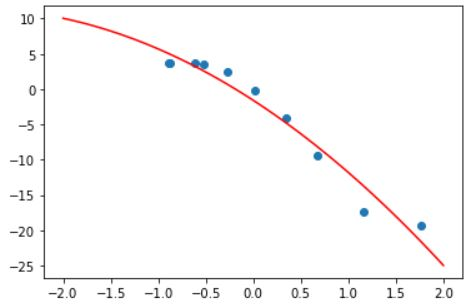
\includegraphics[scale=0.7]{dataset1_10_lambda0_m2funcplot.jpg}
	\caption{    M=2}
	\label{fig:fig1.1.1.1}
	\end{subfigure}
	\hfill
	\begin{subfigure}[b]{0.45\textwidth}
	\centering
	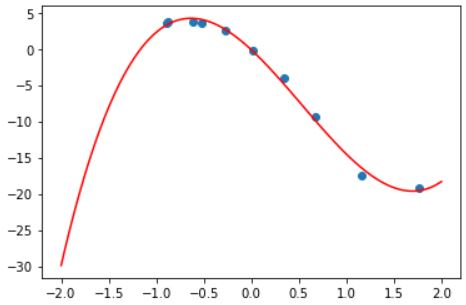
\includegraphics[scale=0.7]{dataset1_10_lambda0_m3funcplot.jpg}
	\caption{    M=3}
	\label{fig:fig1.1.1.2}
	\end{subfigure}
	\hfill
	\begin{subfigure}[b]{0.45\textwidth}
	\centering
	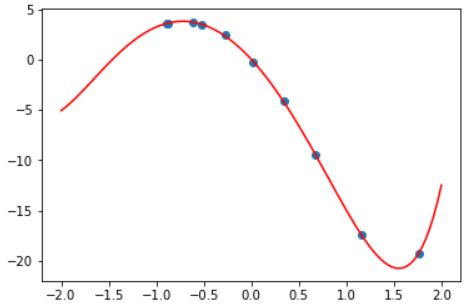
\includegraphics[scale=0.7]{dataset1_10_lambda0_m6funcplot.jpg}
	\caption{    M=6}
	\label{fig:fig1.1.1.3}
	\end{subfigure}
	\hfill
	\begin{subfigure}[b]{0.45\textwidth}
	\centering
	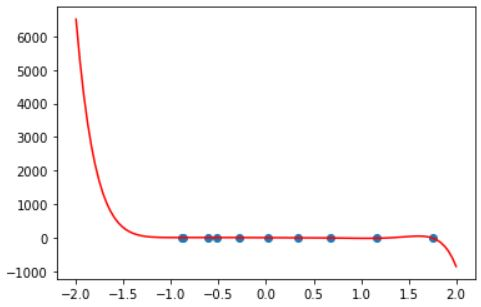
\includegraphics[scale=0.7]{dataset1_10_lambda0_m9funcplot.jpg}
	\caption{    M=9}
	\label{fig:fig1.1.1.4}
	\end{subfigure}
\caption{Approximated function vs Training points for dataset1, training size =10, $\lambda = 0$}
\label{fig:fig1.1.1}
\end{figure}

\newpage

\subsubsection{Datapoints in training dataset - 200}
Hyperparameters $M = \{2,3,6,9\}, \lambda = 0$
\begin{table}[h]
\label{tab:tab1.1.2}
\begin{center}
\begin{tabular}{|l|c|c|c|}
\hline
\textbf{M (Hyperparameter)} & \textbf{Training Dataset} & \textbf{Validation Dataset} &\textbf{Test Dataset}\\
\hline
$2$ & 5.2002 & 4.7814 & 5.4460\\
\hline
$3$ & 1.1704 & 1.1519 & 1.2110\\
\hline
$6$ & 0.0923 & 0.0972 & 0.1087\\
\hline
$9$ & 0.0922 & 0.0974 & 0.1089\\
\hline
\end{tabular}
\caption{ERMS for dataset1, training size = 200, $\lambda = 0$}
\end{center}
\end{table}

\begin{figure}[h]
\centering
	\begin{subfigure}[b]{0.45\textwidth}
	\centering
	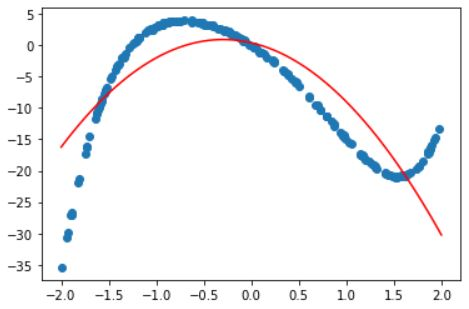
\includegraphics[scale=0.7]{dataset1_200_lambda0_m2funcplot.jpg}
	\caption{    M=2}
	\label{fig:fig1.1.2.1}
	\end{subfigure}
	\hfill
	\begin{subfigure}[b]{0.45\textwidth}
	\centering
	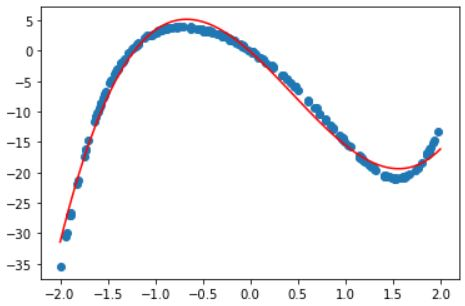
\includegraphics[scale=0.7]{dataset1_200_lambda0_m3funcplot.jpg}
	\caption{    M=3}
	\label{fig:fig1.1.2.2}
	\end{subfigure}
	\hfill
	\begin{subfigure}[b]{0.45\textwidth}
	\centering
	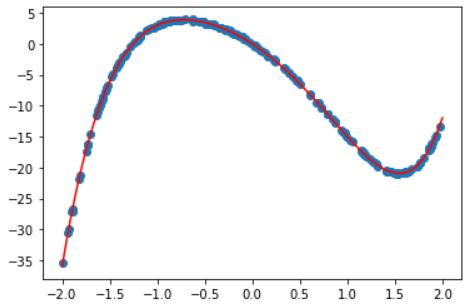
\includegraphics[scale=0.7]{dataset1_200_lambda0_m6funcplot.jpg}
	\caption{    M=6}
	\label{fig:fig1.1.2.3}
	\end{subfigure}
	\hfill
	\begin{subfigure}[b]{0.45\textwidth}
	\centering
	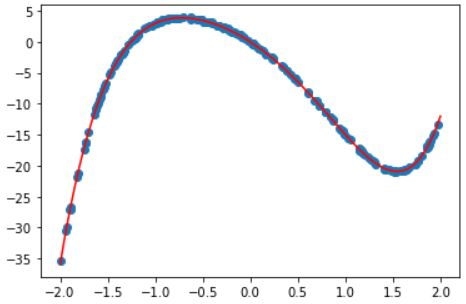
\includegraphics[scale=0.7]{dataset1_200_lambda0_m9funcplot.jpg}
	\caption{    M=9}
	\label{fig:fig1.1.2.4}
	\end{subfigure}
\caption{Approximated function vs Training points for dataset1, training size = 100, $\lambda = 0$}
\label{fig:fig1.1.2}
\end{figure}

\newpage

\subsection{With Regularization}
\subsubsection{Datapoints in training dataset - 10, $\lambda = 0.1$}

Since we observed overfitting only when dataset size was 10 and $M$ was higher.\\
Hyperparameters $M = \{6,9\}, \lambda = 0.1$
\begin{table}[h]
\label{tab:tab1.2.1}
\begin{center}
\begin{tabular}{|l|c|c|c|}
\hline
\textbf{M (Hyperparameter)} & \textbf{Training Dataset} & \textbf{Validation Dataset} &\textbf{Test Dataset}\\
\hline
$6$ & 0.3900 & 0.9661 & 1.7154\\
\hline
$9$ & 0.4045 & 28.8458 & 35.8129\\
\hline
\end{tabular}
\caption{ERMS for dataset1, training size =10, $\lambda = 0.1$}
\end{center}
\end{table}

\begin{figure}[h]
\centering
	\begin{subfigure}[b]{0.4\textwidth}
	\centering
	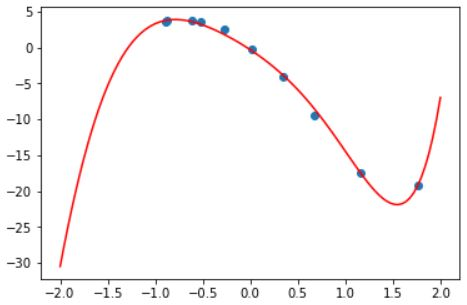
\includegraphics[scale=0.7]{dataset1_10_lambda1_m6funcplot.jpg}
	\caption{    M=6}
	\label{fig:fig1.2.1.1}
	\end{subfigure}
	\hfill
	\begin{subfigure}[b]{0.4\textwidth}
	\centering
	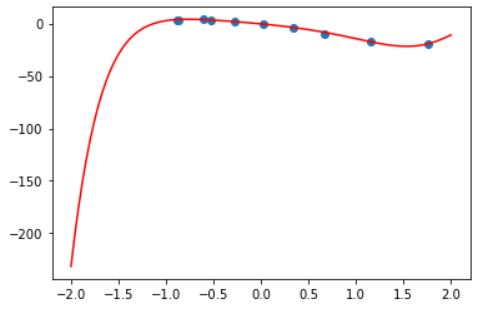
\includegraphics[scale=0.7]{dataset1_10_lambda1_m9funcplot.jpg}
	\caption{    M=9}
	\label{fig:fig1.2.1.2}
	\end{subfigure}
\caption{Approximated function vs Training points for dataset1, training size =10, $\lambda = 0.1$}
\label{fig:fig1.2.1}
\end{figure}

\textbf{Observations :}\\
We observed in the section that when we don't have enough data for training i.e when we had only 10 points for training and the model complexity is high, the ERMS for training data is pretty low although the ERMS for test and validation is higher. This is because of overfitting and when we have more data i.e 200 points for training and the model complexity is high this problem is resolved.
\newpage

\section{Linear model for regression using Polynomial Basis function}
Dataset2 : function2-2d.csv is used for all the experiments in the given section.
\subsection{Without regularization}
\subsubsection{Datapoints in training dataset - 50}
Hyperparameters $M = \{2,3,6\}$
\begin{table}[h]
\label{tab:tab2.1.1}
\begin{center}
\begin{tabular}{|l|c|c|c|}
\hline
\textbf{M (Hyperparameter)} & \textbf{Training Dataset} & \textbf{Validation Dataset} &\textbf{Test Dataset}\\
\hline
$2$ & $1.5604*10^{-13}$ & $1.5524*10^{-13}$ & $2.0963*10^{-13}$\\
\hline
$3$ & $4.6330*10^{-13}$ & $5.5056*10^{-13}$ & $7.7062*10^{-13}$\\
\hline
$6$ & $2.1917*10^{-10}$ & $7.3972*10^{-10}$ & $2.8797*10^{-10}$\\
\hline
\end{tabular}
\caption{ERMS for dataset2, training size = 50, $\lambda = 0$}
\end{center}
\end{table}

\begin{figure}[h]
\centering
	\begin{subfigure}[b]{0.4\textwidth}
	\centering
	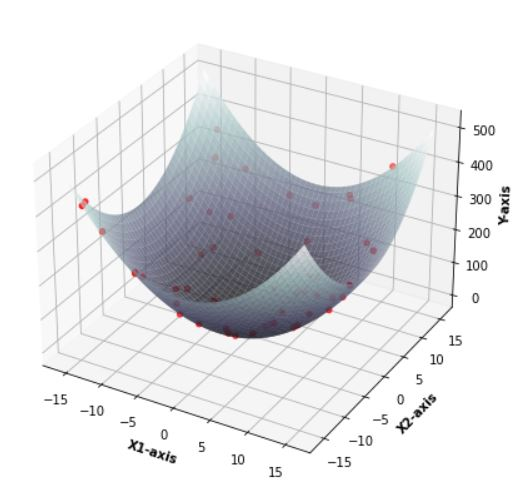
\includegraphics[scale=0.5]{dataset2_50_lambda0_m2funcplot.jpg}
	\caption{    M=2}
	\label{fig:fig2.1.1.1}
	\end{subfigure}
	\hfill
	\begin{subfigure}[b]{0.4\textwidth}
	\centering
	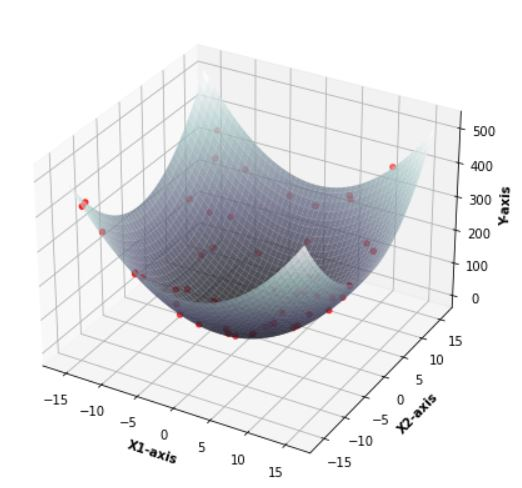
\includegraphics[scale=0.5]{dataset2_50_lambda0_m3funcplot.jpg}
	\caption{    M=3}
	\label{fig:fig2.1.1.2}
	\end{subfigure}
	\hfill
	\begin{subfigure}[b]{0.4\textwidth}
	\centering
	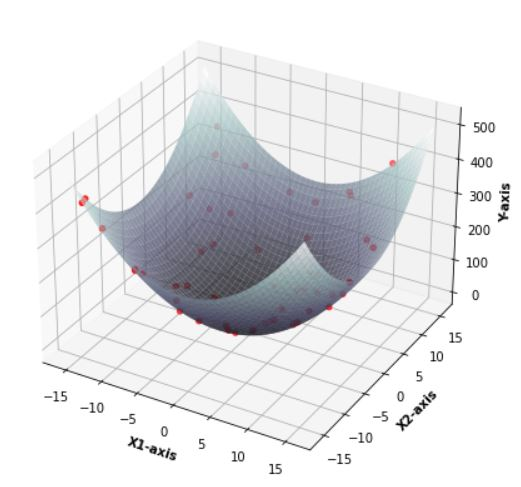
\includegraphics[scale=0.5]{dataset2_50_lambda0_m6funcplot.jpg}
	\caption{    M=6}
	\label{fig:fig2.1.1.3}
	\end{subfigure}
\caption{Approximated surface vs Training points for dataset2, training size = 50, $\lambda = 0$}
\label{fig:fig2.1.1}
\end{figure}

\newpage
\subsubsection{Datapoints in training dataset - 200}
Hyperparameters $M = \{2,3,6\}$
\begin{table}[h]
\label{tab:tab2.1.3}
\begin{center}
\begin{tabular}{|l|c|c|c|}
\hline
\textbf{M (Hyperparameter)} & \textbf{Training Dataset} & \textbf{Validation Dataset} &\textbf{Test Dataset}\\
\hline
$2$ & $1.2609*10^{-13}$ & $1.1539*10^{-13}$ & $1.2662*10^{-13}$\\
\hline
$3$ & $6.9699*10^{-13}$ & $7.4280*10^{-13}$ & $7.2801*10^{-13}$\\
\hline
$6$ & $2.2037*10^{-10}$ & $2.1976*10^{-10}$ & $2.1677*10^{-10}$\\
\hline
\end{tabular}
\caption{ERMS for dataset2, training size = 200, $\lambda = 0$}
\end{center}
\end{table}

\begin{figure}[h]
\centering
	\begin{subfigure}[b]{0.4\textwidth}
	\centering
	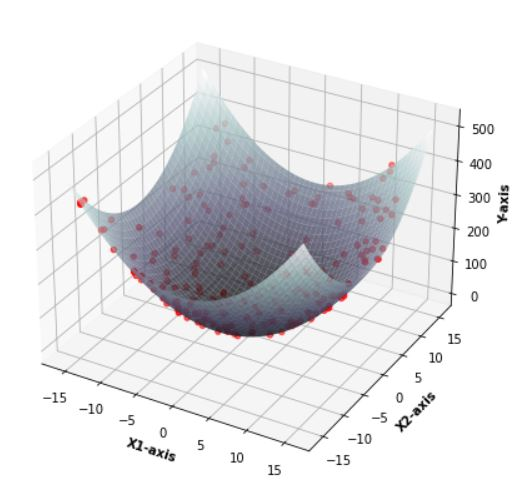
\includegraphics[scale=0.5]{dataset2_200_lambda0_m2funcplot.jpg}
	\caption{    M=2}
	\label{fig:fig2.1.3.1}
	\end{subfigure}
	\hfill
	\begin{subfigure}[b]{0.4\textwidth}
	\centering
	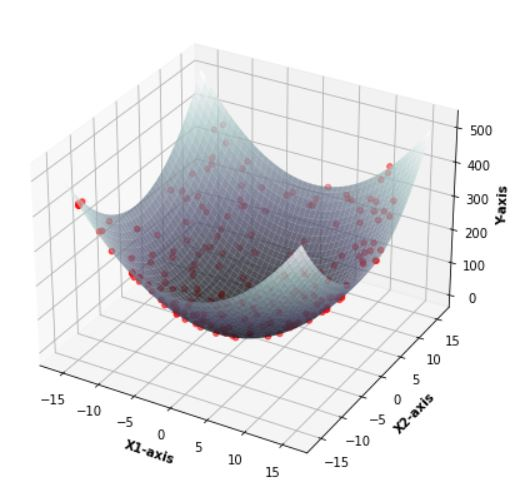
\includegraphics[scale=0.5]{dataset2_200_lambda0_m3funcplot.jpg}
	\caption{    M=3}
	\label{fig:fig2.1.3.2}
	\end{subfigure}
	\hfill
	\begin{subfigure}[b]{0.4\textwidth}
	\centering
	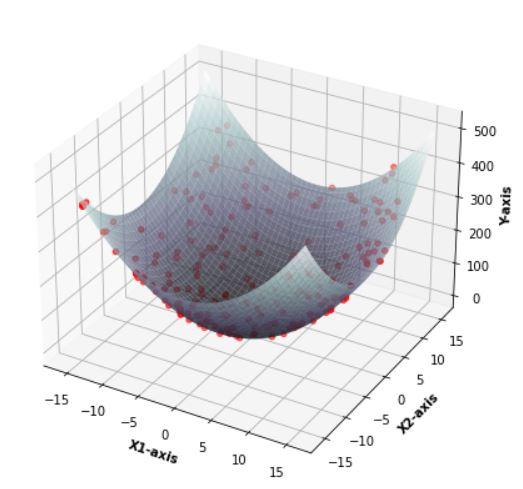
\includegraphics[scale=0.5]{dataset2_200_lambda0_m6funcplot.jpg}
	\caption{    M=6}
	\label{fig:fig2.1.3.3}
	\end{subfigure}
\caption{Approximated surface vs Training points for dataset2, training size = 200, $\lambda = 0$}
\label{fig:fig2.1.3}
\end{figure}
\newpage

\subsubsection{Datapoints in training dataset - 500}
Hyperparameters $M = \{2,3,6\}$
\begin{table}[h]
\label{tab:tab2.1.3}
\begin{center}
\begin{tabular}{|l|c|c|c|}
\hline
\textbf{M (Hyperparameter)} & \textbf{Training Dataset} & \textbf{Validation Dataset} &\textbf{Test Dataset}\\
\hline
$2$ & $2.0275*10^{-13}$ & $2.0586*10^{-13}$ & $2.0963*10^{-13}$\\
\hline
$3$ & $7.9449*10^{-13}$ & $7.4680*10^{-13}$ & $7.7062*10^{-13}$\\
\hline
$6$ & $3.1754*10^{-10}$ & $2.8852*10^{-10}$ & $2.8797*10^{-10}$\\
\hline
\end{tabular}
\caption{ERMS for dataset2, training size = 500, $\lambda = 0$}
\end{center}
\end{table}

\begin{figure}[h]
\centering
	\begin{subfigure}[b]{0.4\textwidth}
	\centering
	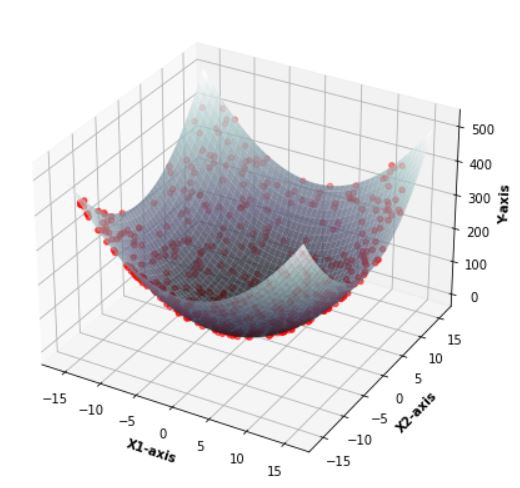
\includegraphics[scale=0.5]{dataset2_500_lambda0_m2funcplot.jpg}
	\caption{    M=2}
	\label{fig:fig2.1.3.1}
	\end{subfigure}
	\hfill
	\begin{subfigure}[b]{0.4\textwidth}
	\centering
	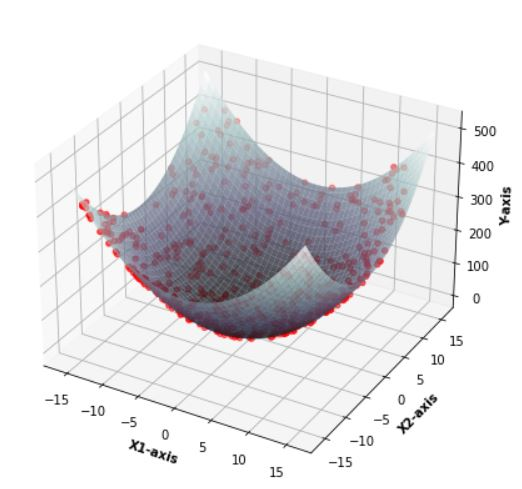
\includegraphics[scale=0.5]{dataset2_500_lambda0_m3funcplot.jpg}
	\caption{    M=3}
	\label{fig:fig2.1.3.2}
	\end{subfigure}
	\hfill
	\begin{subfigure}[b]{0.4\textwidth}
	\centering
	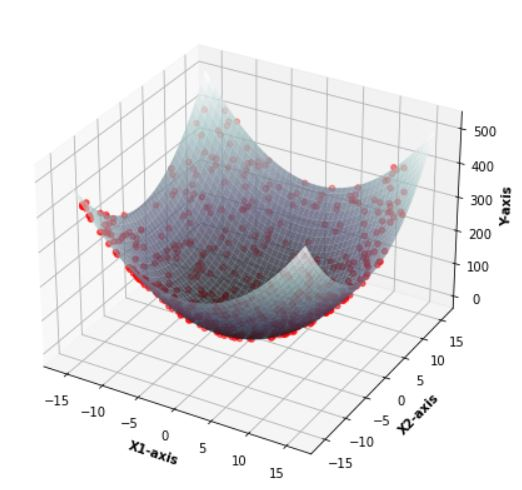
\includegraphics[scale=0.5]{dataset2_500_lambda0_m6funcplot.jpg}
	\caption{    M=6}
	\label{fig:fig2.1.3.3}
	\end{subfigure}
\caption{Approximated surface vs Training points for dataset2, training size = 500, $\lambda = 0$}
\label{fig:fig2.1.3}
\end{figure}

We see that for none of the cases the model complexity is too high for the amount of training data available and hence we don't require and regularization.
\newpage

\subsubsection{Scatter plots, training size = 50}
\begin{figure}[h]
\centering
	\begin{subfigure}[b]{0.4\textwidth}
	\centering
	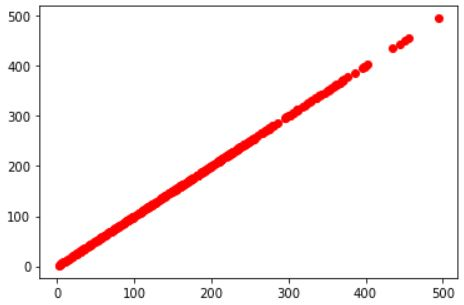
\includegraphics[scale=0.5]{dataset2_50_lambda0_test.jpg}
	\caption{Testing Data}
	\label{fig:fig2.1.4.1}
	\end{subfigure}
	\hfill
	\begin{subfigure}[b]{0.4\textwidth}
	\centering
	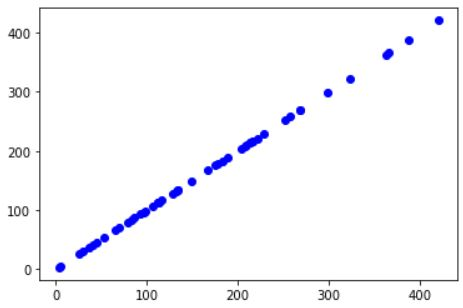
\includegraphics[scale=0.5]{dataset2_50_lambda0_train.jpg}
	\caption{Training Data}
	\label{fig:fig2.1.4.2}
	\end{subfigure}
\caption{Model output vs Target output for dataset2, training size = 50, $\lambda = 0$, $M =2 $}
\label{fig:fig2.1.4}
\end{figure}

\subsubsection{Scatter plots, training size = 200}
\begin{figure}[h]
\centering
	\begin{subfigure}[b]{0.4\textwidth}
	\centering
	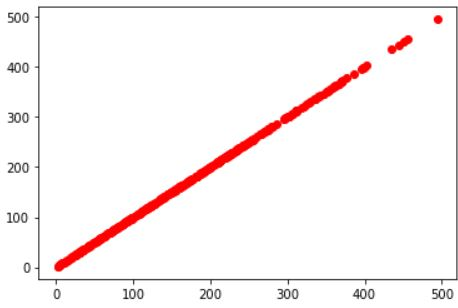
\includegraphics[scale=0.5]{dataset2_200_lambda0_test.jpg}
	\caption{Testing Data}
	\label{fig:fig2.1.5.1}
	\end{subfigure}
	\hfill
	\begin{subfigure}[b]{0.4\textwidth}
	\centering
	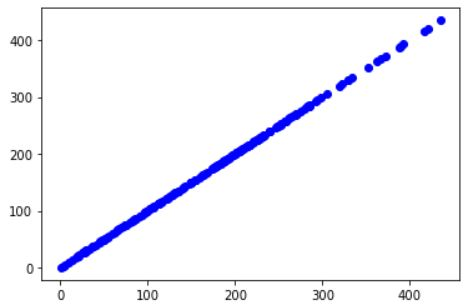
\includegraphics[scale=0.5]{dataset2_200_lambda0_train.jpg}
	\caption{Training Data}
	\label{fig:fig2.1.5.2}
	\end{subfigure}
\caption{Model output vs Target output for dataset2, training size = 200, $\lambda = 0$, $M =2 $}
\label{fig:fig2.1.5}
\end{figure}

\subsubsection{Scatter plots, training size = 500}
\begin{figure}[h]
\centering
	\begin{subfigure}[b]{0.4\textwidth}
	\centering
	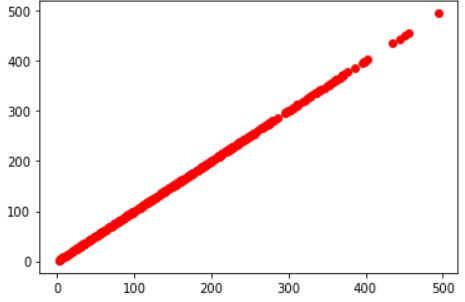
\includegraphics[scale=0.5]{dataset2_500_lambda0_test.jpg}
	\caption{Testing Data}
	\label{fig:fig2.1.6.1}
	\end{subfigure}
	\hfill
	\begin{subfigure}[b]{0.4\textwidth}
	\centering
	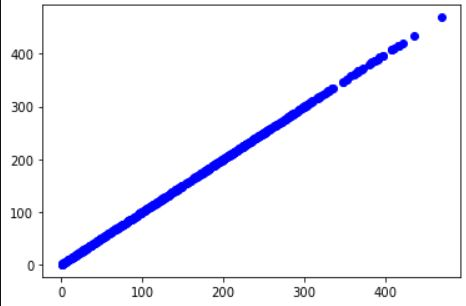
\includegraphics[scale=0.5]{dataset2_500_lambda0_train.jpg}
	\caption{Training Data}
	\label{fig:fig2.1.6.2}
	\end{subfigure}
\caption{Model output vs Target output for dataset2, training size = 500, $\lambda = 0$, $M =3 $}
\label{fig:fig2.1.6}
\end{figure}

\newpage
\section{Linear model for regression using Gaussian Basis function}

For Task 3 the amount of data to be taken for training was not mentioned specifically so we took 70\% of the available data as training data.
\subsection{Dataset 2 : function2-2d.csv}
\subsubsection{Without regularization}
Hyperparameters : $\sigma = 20 $, K = Number of clusters = $\{20,22,24\}$

\begin{table}[h]
\label{tab:tab3.1.1}
\begin{center}
\begin{tabular}{|l|c|c|c|}
\hline
\textbf{K } & \textbf{Training Dataset}&\textbf{Validation Dataset} & \textbf{Test Dataset} \\
\hline
$20$ & 3.2877 & 4.0803 & 4.9529\\
\hline
$22 $ & 3.0172 & 3.2468 & 3.6907\\
\hline
$24$ (Best) & 2.5483 & 2.9303 & 3.1383\\
\hline
\end{tabular}
\caption{ERMS for dataset2, $\lambda = 0$, $\sigma = 20$}
\end{center}
\end{table}

\begin{figure}[h]
\centering
	\begin{subfigure}[b]{0.45\textwidth}
	\centering
	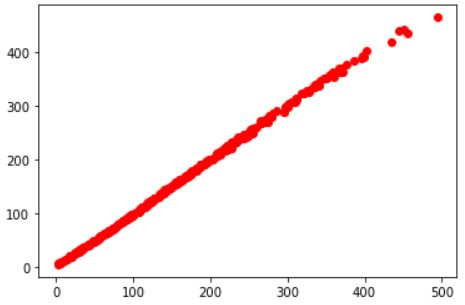
\includegraphics[scale=0.7]{dataset2_k8_lambda0_test.jpg}
	\caption{Testing Data}
	\label{fig:fig3.1.1.1}
	\end{subfigure}
	\begin{subfigure}[b]{0.45\textwidth}
	\centering
	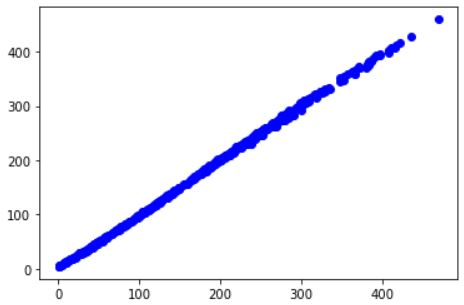
\includegraphics[scale=0.7]{dataset2_k8_lambda0_train.jpg}
	\caption{Training Data}
	\label{fig:fig3.1.1.2}
	\end{subfigure}
\caption{Model output vs Target output for dataset2, $\lambda =0$, $\sigma =20$, $K = 24$}
\label{fig:fig3.1.1}
\end{figure}

As we can see there is no overfitting observed since we already have enough data even for model with higher complexities like with $K =24$. Hence no regularization is required.

\newpage
\subsection{Dataset 3 : 2-music.txt}

We applied feature scaling on the inputs to improve the model efficiency.\\

\subsubsection{Without regularization}
Hyperparameters : $\sigma = 250$; K = Number of clusters = $\{3,5,8,10\}$
\begin{table}[h]
\label{tab:tab3.2.1}
\begin{center}
\begin{tabular}{|l|c|c|c|}
\hline
\textbf{K} & \textbf{Training Dataset} & \textbf{Test Dataset} &\textbf{Validation Dataset}\\
\hline
 $3$ & 0.054272 & 0.062679 & 0.043885\\
\hline
 $5$ & 0.047456 & 0.050827 & 0.036754\\
\hline
 $8 $ & 0.021510 & 0.023942 & 0.019601\\
\hline
 $10 (Best) $ & 0.016433 & 0.015821 & 0.013432\\
\hline
\end{tabular}
\caption{ERMS for dataset 3, $\lambda = 0$}
\end{center}
\end{table}

\begin{figure}[h]
\centering
	\begin{subfigure}[b]{0.4\textwidth}
	\centering
	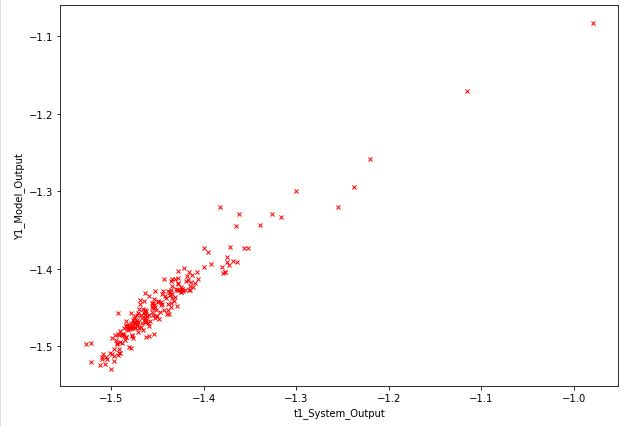
\includegraphics[scale=0.35]{dataset3_k10_lambda0_test1.jpg}
	\caption{Testing Data, $y1$}
	\label{fig:fig3.2.1.1}
	\end{subfigure}
	\hfill
	\begin{subfigure}[b]{0.4\textwidth}
	\centering
	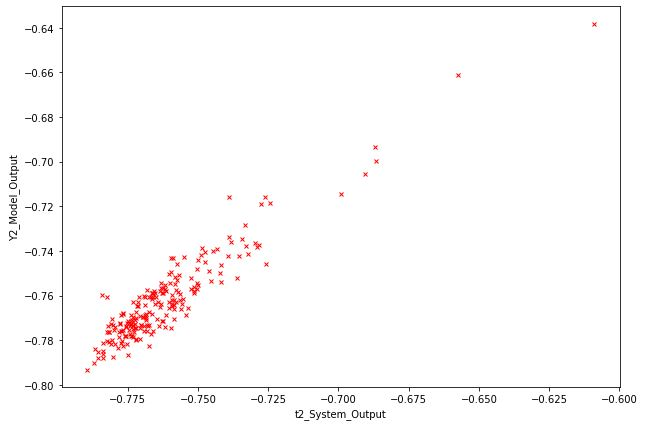
\includegraphics[scale=0.35]{dataset3_k10_lambda0_test2.jpg}
	\caption{Testing Data,$y2$}
	\label{fig:fig3.2.1.2}
	\end{subfigure}
	\hfill
	\begin{subfigure}[b]{0.4\textwidth}
	\centering
	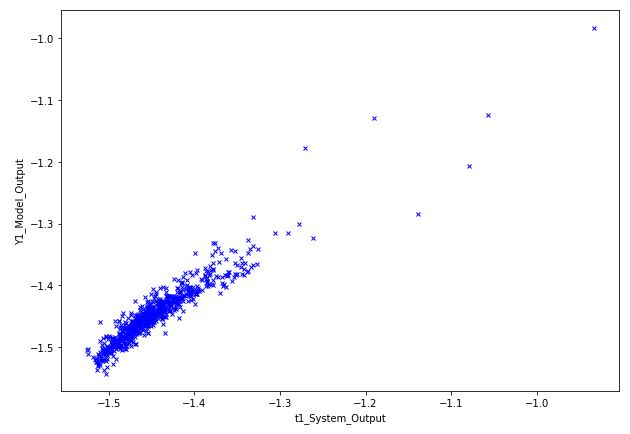
\includegraphics[scale=0.35]{dataset3_k10_lambda0_train1.jpg}
	\caption{Training Data,$y1$}
	\label{fig:fig3.2.1.3}
	\end{subfigure}
	\hfill
	\begin{subfigure}[b]{0.4\textwidth}
	\centering
	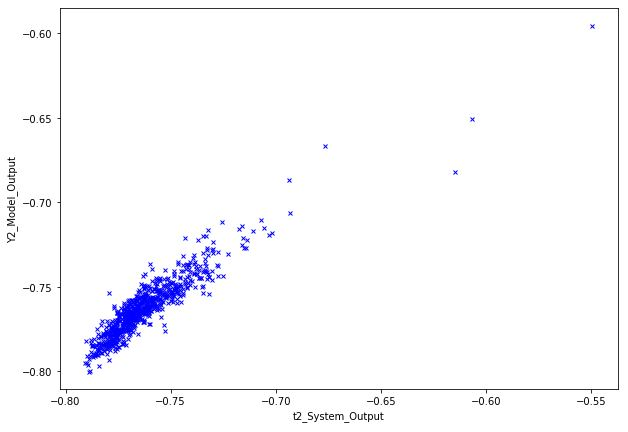
\includegraphics[scale=0.35]{dataset3_k10_lambda0_train2.jpg}
	\caption{Training Data,$y2$}
	\label{fig:fig3.2.1.4}
	\end{subfigure}
\caption{Model output vs Target output for dataset 3, $\lambda = 0$}
\label{fig:fig3.2.1}
\end{figure}

\textbf{Observation :} \\
Here since we were using 70\% of the data we had the liberty to go for a complex model i.e. for higher value of K with the performance of model still increasing at a good rate.
\end{document}
